\documentclass[french]{article}
%\usepackage[utf8]{inputenc}
\usepackage[T1]{fontenc}
\usepackage[a4paper,top=0.8in, bottom=1.0in, left=1.0in, right=1.25in]{geometry}
%\usepackage{babel}
\usepackage{graphicx}
\usepackage{amsmath}
\usepackage{cleveref}
%\usepackage{fancybox}
%\usepackage{framed}

\title{ \textbf{Two DOF planar robot model predictive control }  }
\author{\textit{\textbf{R.B. Ashith Shyam}}}
\date{}

\begin{document}
	\maketitle
\section{Equation of motion in state-space}

\begin{figure}[h]
	\centering
	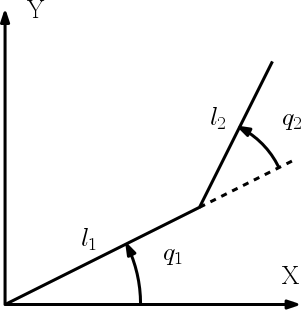
\includegraphics[width=0.3\linewidth, height=0.15\textheight]{2r_schematic}
	\caption{Schematic of a planar 2-DOF robot}
	\label{fig:2rschematic}
\end{figure}


	
	The equation of motion of a 2R planar robot can be expressed as 
	\begin{align}
	[M]\begin{bmatrix}
	\ddot{q}_1 \\ 
	\ddot{q}_2
	\end{bmatrix} + C + G = \begin{bmatrix}
	u_1 \\ 
	u_2
	\end{bmatrix}
	\end{align}
	where $q_i's$ and $ u_i's$, i = 1, 2 are the joint angles and the input torques in joint space \\
	In state-space form this can be written as ($q_1 ~= ~x_1,~ q_2 ~= ~x_2,~ \dot{q}_1 ~=~ ~x_3$ and $\dot{q}_2~ = ~x_4$)	
	\begin{align}
	\dot{X} = \begin{bmatrix}
	\dot{x}_1 \\ 
	\dot{x}_2 \\ 
	\dot{x}_3 \\ 
	\dot{x}_4
	\end{bmatrix} = \begin{bmatrix}
	x_3 \\ 
	x_4 \\ 
	M^{-1}\Big[\begin{pmatrix}
	u_1 \\ 
	u_2
	\end{pmatrix} - C - G\Big]
	\end{bmatrix} 
			\label{eq:feedback_linearization}
	\end{align}
	\section{Feedback Linearization}
	\begin{align}
	\begin{bmatrix}
	u_1 \\ 
	u_2
	\end{bmatrix} = \alpha \begin{bmatrix}
	u_1' \\ 
	u_2'
	\end{bmatrix} + \beta
	\end{align}
	Choose $\alpha = M$ and $\beta = ~ C + G$, \cref{eq:feedback_linearization} becomes
	%
	\begin{align}
	\dot{X} = \begin{bmatrix}
	\dot{x}_1 \\ 
	\dot{x}_2 \\ 
	\dot{x}_3 \\ 
	\dot{x}_4
	\end{bmatrix} = \begin{bmatrix}
	0 & 0 & 1 & 0 \\ 
	0 & 0 & 0 & 1 \\ 
	0 & 0 & 0 & 0 \\ 
	0 & 0 & 0 & 0
	\end{bmatrix} \begin{bmatrix}
	{x}_1 \\ 
	{x}_2 \\ 
	{x}_3 \\ 
	{x}_4
	\end{bmatrix} + \begin{bmatrix}
	0 & 0 \\ 
	0 & 0 \\ 
	1 & 0 \\ 
	0 & 1
	\end{bmatrix} \begin{bmatrix}
	u_1 \\ 
	u_2
	\end{bmatrix} 
	\end{align}
	To track the joint angles, the output equation becomes
	\begin{align}
	Y = \begin{pmatrix}
	x_1 \\ 
	x_2
	\end{pmatrix} = \begin{bmatrix}
	1 & 0 & 0 & 0 \\ 
	0 & 1 & 0 & 0
	\end{bmatrix} \begin{bmatrix}
	{x}_1 \\ 
	{x}_2 \\ 
	{x}_3 \\ 
	{x}_4
	\end{bmatrix}
	\end{align}
	So the linearized system dynamics becomes,
	\begin{align}
	\dot{X} &= A~ X + B~ U \nonumber\\
	Y &= C~ X
	\end{align}
	where 
	\begin{align}
	A = \begin{bmatrix}
	0 & 0 & 1 & 0 \\ 
	0 & 0 & 0 & 1 \\ 
	0 & 0 & 0 & 0 \\ 
	0 & 0 & 0 & 0
	\end{bmatrix}, B = \begin{bmatrix}
	1 & 0 & 0 & 0 \\ 
	0 & 1 & 0 & 0
	\end{bmatrix}, X = \begin{pmatrix}
	{x}_1 \\ 
	{x}_2 \\ 
	{x}_3 \\ 
	{x}_4
	\end{pmatrix} \rm{and} ~U = \begin{pmatrix}
	u_1 \\ 
	u_2
	\end{pmatrix}
	\end{align}
	\section{Output trajectory tracking by MPC}
	Let $y_r$ be the reference trajectory the tip of the end-effector should follow, N be the prediction horizon, the cost function, J, can be written as
	\begin{align}
	J &= (y_{N/k} - y_r)^T P' (y_{N/k} - y_r) + \sum_{i=0}^{N-1} (y_{i/k} - y_r)^T Q' (y_{i/k} - y_r) + u_{i/k}^T R u_{i/k} \\
	%
	&= (Cx_{N/k} - y_r)^T P' (Cx_{N/k} - y_r) + \sum_{i=0}^{N-1} (Cx_{i/k} - y_r)^T Q' (Cx_{i/k} - y_r) + u_{i/k}^T R u_{i/k}	\nonumber \\
	%
	&= x_{N/k}^T C^TP'C x_{N/k} -  2 x_{N/k}^T C^TP' y_r + y_r^TP'y_r + \sum_{i=0}^{N-1} x_{i/k}^T C^TQ'C x_{i/k} - 2 x_{i/k}^TC^TQ'y_r + y_r^TQ'y_r + u_{i/k}^T R u_{i/k}
	\end{align}
	where P', Q', R are penalties.
	This can be further simplified and can be written as
	\begin{multline}
		J = y_r^TP'y_r + x_{0/k}^T Q x_{0/k} - 2 x_{0/k} Qd y_r + \begin{pmatrix}
			x_1 \\ 
			x_2 \\ 
			: \\ 
			: \\ 
			x_N
		\end{pmatrix}^T_k \begin{bmatrix}
			Q &  &  &  &  \\ 
			& Q &  &  &  \\ 
			&  & : &  &  \\ 
			&  &  & : &  \\ 
			&  &  &  & P
		\end{bmatrix} \begin{pmatrix}
			x_1 \\ 
			x_2 \\ 
			: \\ 
			: \\ 
			x_N
		\end{pmatrix}_k - 2 \begin{pmatrix}
			x_1 \\ 
			x_2 \\ 
			: \\ 
			: \\ 
			x_N
		\end{pmatrix}^T_k \begin{bmatrix}
			Qd &  &  &  &  \\ 
			& Qd &  &  &  \\ 
			&  & : &  &  \\ 
			&  &  & : &  \\ 
			&  &  &  & Pd
		\end{bmatrix} \begin{pmatrix}
			y_r \\ 
			y_r \\ 
			: \\ 
			: \\ 
			y_r
		\end{pmatrix}_k \\
		%
	+	\begin{pmatrix}
		u_0 \\ 
		u_1 \\ 
		: \\ 
		: \\ 
		u_{N-1}
		\end{pmatrix}^T_k \begin{bmatrix}
		R &  &  &  &  \\ 
		& R &  &  &  \\ 
		&  & : &  &  \\ 
		&  &  & : &  \\ 
		&  &  &  & R
		\end{bmatrix} \begin{pmatrix}
		u_0 \\ 
		u_1 \\ 
		: \\ 
		: \\ 
		u_{N-1}
		\end{pmatrix}_k \nonumber
	\end{multline}
\begin{align}
	J = y_r^TP'y_r + x_{0/k}^T~ Qd~ x_{0/k} - 2 x_{0/k} Q y_r + X_k^T F X_k - 2 X_k^T G y_{r_k} + U_k^T H U_k
	\label{eq:costfunction}
\end{align}
where P = $C^TP'C$, Pd = $C^TP'$, Q = $C^TQ'C$, Qd = $C^TQ'$, F = $\begin{bmatrix}
Q &  &  &  &  \\ 
& Q &  &  &  \\ 
&  & : &  &  \\ 
&  &  & : &  \\ 
&  &  &  & P
\end{bmatrix} $, G = $\begin{bmatrix}
	Qd &  &  &  &  \\ 
	& Qd &  &  &  \\ 
	&  & : &  &  \\ 
	&  &  & : &  \\ 
	&  &  &  & Pd
\end{bmatrix} $, H = $\begin{bmatrix}
R &  &  &  &  \\ 
& R &  &  &  \\ 
&  & : &  &  \\ 
&  &  & : &  \\ 
&  &  &  & R
\end{bmatrix} $ and $Y_R =  \begin{pmatrix}
	y_r \\ 
	y_r \\ 
	: \\ 
	: \\ 
	y_r
\end{pmatrix}_k$

For a control horizon of N, we can write the following for the k$^th$ sampling time
\begin{align*}
	x_1 &= A x_0 + B u_0 \\
	x_2 &= A x_1 + B u_1 = A\Big(A x_0 + B u_0\Big) + B u_1 = A^2 x_0 + ABu_0 + Bu_1\\
	 :\\
	 :\\
	x_N &= A x_{N-1} + B u_{N-1} = A^N x_0 + A^{N-2}B u_1 + A^{N-3}Bu_2 +...Bu_{N-1}\\
	\begin{pmatrix}
	x_1 \\ 
	x_2 \\ 
	: \\ 
	: \\ 
	x_N
	\end{pmatrix}_k &= \begin{pmatrix}
	A \\ 
	A^2 \\ 
	: \\ 
	: \\ 
	A^N
	\end{pmatrix} x_0 + \begin{bmatrix}
	B & 0 & .... & 0 \\ 
	AB & B & .... & 0 \\ 
	: & : & .... & : \\ 
	: & : & .... & : \\ 
	A^{N-1}B & A^{N-2}B & .... & B
	\end{bmatrix} \begin{pmatrix}
	u_0 \\ 
	u_1 \\ 
	: \\ 
	: \\ 
	u_{N-1}
	\end{pmatrix}_k \\
\end{align*}
\begin{align}
	X_k &= S_x x_0 + S_u U_k
	\label{eq:prediction_model}
\end{align}
Substituting \cref{eq:prediction_model} in \cref{eq:costfunction}, the cost becomes
\begin{align}
	J = y_r^TP'y_r + x_{0/k}^T~ Qd~ x_{0/k} - 2 x_{0/k} Q y_r + (S_x x_0 + S_u U_k)^T F (S_x x_0 + S_u U_k) - 2 (S_x x_0 + S_u U_k)^T G y_{r_k} + U_k^T H U_k
\end{align}
\textbf{Since $U_k$ is the variable for optimization, the terms independent of $U_k$ can be omitted in the cost function}
\begin{align}
	J &= U_k^T (2S_u^TFS_x) x_0 + U_k^T(S_u^TFS_u + H)U_k - U_k^T (2S_u^TG) Y_R \nonumber \\
	&= \frac 12 U_k^T W U_k + U_k^T K x_0 - U_k^T L Y_R
\end{align}
where W = 2 $(S_u^TFS_u + H)$, K = $2S_u^TFS_x$ and L = $2S_u^TG$
\end{document}


